\documentclass{sfuthesis}

\title{More on kernel contraction in $\mathcal{EL}$}
\thesistype{Dissertation}
\author{Amr Dawood}
\previousdegrees{%
	B.Sc., German University in Cairo, 2011}
\degree{Master of Science}
\discipline{Computing Science}
\department{Department of Computing Science}
\faculty{Faculty of Applied Sciences}
\copyrightyear{2015}
\semester{Fall 2015}
\date{1 September 2015}

\keywords{Masters; Thesis; Simon Fraser University; Kernel Contraction; EL; Description Logic; Specificity; Localization}

\committee{%
	\chair{name}{Professor}
	\member{James P. Delgrande}{Senior Supervisor\\Professor}
	\member{David G. Mitchell}{Supervisor\\Associate Professor}
}

%   PACKAGES AND CUSTOMIZATIONS  %%%%%%%%%%%%%%%%%%%%%%%%%%%%%%%%%%%%%%%%%%%%%%
%
%   Add any packages or custom commands you need for your thesis here.
%   You don't need to call the following packages, which are already called in
%   the sfuthesis class file:
%
%   - appendix
%   - etoolbox
%   - fontenc
%   - geometry
%   - lmodern
%   - nowidow
%   - setspace
%   - tocloft
%
%   If you call one of the above packages (or one of their dependencies) with
%   options, you may get a "Option clash" LaTeX error. If you get this error,
%   you can fix it by removing your copy of \usepackage and passing the options
%   you need by adding
%
%       \PassOptionsToPackage{<options>}{<package>}
%
%   before \documentclass{sfuthesis}.
%

\usepackage{amsmath,amssymb,amsthm}
\usepackage[pdfborder={0 0 0}]{hyperref}
\usepackage{graphicx}
\usepackage{caption}
\usepackage{algorithm}
\usepackage{algpseudocode}


\theoremstyle{plain}
\newtheorem{thm}{Theorem}[chapter]
\theoremstyle{definition}
\newtheorem{defn}[thm]{Definition}



%   FRONTMATTER  %%%%%%%%%%%%%%%%%%%%%%%%%%%%%%%%%%%%%%%%%%%%%%%%%%%%%%%%%%%%%%
%
%   Title page, committee page, copyright declaration, abstract,
%   dedication, acknowledgements, table of contents, etc.
%

\begin{document}

\frontmatter
\maketitle{}
\makecommittee{}

\begin{abstract}
	This is a blank document from which you can start writing your thesis.
\end{abstract}


\begin{dedication} % optional
\end{dedication}


\begin{acknowledgements} % optional
\end{acknowledgements}

\addtoToC{Table of Contents}\tableofcontents\clearpage
\addtoToC{List of Tables}\listoftables\clearpage
\addtoToC{List of Figures}\listoffigures





%   MAIN MATTER  %%%%%%%%%%%%%%%%%%%%%%%%%%%%%%%%%%%%%%%%%%%%%%%%%%%%%%%%%%%%%%
%
%   Start writing your thesis --- or start \include ing chapters --- here.
%
%%%%%%%%%%%%%%%%%%%%%%%%%%%%%%%%%%%%%%%%%%%%%%%%%%%%%%%%%%%%%%

\mainmatter%



\chapter{Introduction}

Changing one's mind is a process that happens very frequently as part of one's daily routine. Seeing the sunrise in the morning, one would intuitively change his mind and believe that it is not dark any more; that would logically imply that one gives up the current belief that it is dawn time and replace it with a new belief that it is sunrise time. This is an example of belief revision. Revision is a kind of change in which the new belief (``it is sunrise'') is conflicting with the current state of mind (believing that ``it is dawn''). 

Mind changing can be thought of as the manipulation of beliefs according to perception. When humans perceive any change in their world, they change their knowledge accordingly. So changing the knowledge (or beliefs\footnote{Throughout this study we will be using the terms ``knowledge'' and ``beliefs'' interchangeably, although they are not exactly the same. Knowledge is usually assumed to be a special kind of beliefs. However, for convenience, when we use the word ``knowledge'' we will be referring to ``belief.'' }) of an agent\footnote{The word ``agent'' here means humans, computers, or any thing that has knowledge base and perception.} can be seen as what we informally call changing the mind of the agent. One example of belief change is \textbf{Revision}, which involves changing the knowledge base in order to add a conflicting belief. This can actually be broken down into two processes: changing the knowledge base to account for the conflict, and adding the new belief. 

The first process involves removing the beliefs that are causing that conflict. This process is called \textbf{Belief Contraction}. The second process involves adding the new belief and expanding the knowledge base accordingly. This process is called \textbf{Belief Expansion}. Contraction is the type of change we are mainly concerned with in this study. Kernel contraction is one approach to contraction that performs by getting all kernels and removing some statements from each of them. 

\section{Kernel contraction by example}
The following chapters will explain kernel contraction in more details, but it is helpful to get a brief idea on what it is before moving on. A kernel is a minimal set of beliefs that imply a certain belief. If our knowledge contains the following beliefs:
\begin{itemize}
\item We are in Canada
\item The trees are green
\item The temperature is 30 Celsius,
\end{itemize}
and we know that whenever these three statements are true then ``it is summer,'' we can imply that it is indeed summer time. In this case, the three beliefs together form a kernel that implies ``it is summer.'' That kernel can be used for contraction purpose. If we want to give up the belief ``it is summer,'' we can remove a belief from the kernel so that the remaining two cannot be enough to imply that it is summer. In some other cases we can have more than one kernel, and the same rules can still apply: remove a belief from each kernel in order to perform kernel contraction. The beliefs used in this example are quite subjective, but the aim is to give a brief and simple example. The following chapters will talk more formally about kernel contraction.

\section{The language}
The knowledge of an agent can be represented as a set of beliefs. An agent is assumed to believe in $A$ if $A$ is a member of its \textit{belief set}\footnote{Belief sets will be explained in the next chapter}. In this study, the language used to represent belief sets is \textit{Description Logic}. Description Logic is a family of formalisms that are used to represent knowledge. They use concepts to represent classes of individuals and roles to represent relationships between them. They have different expressive powers and different reasoning mechanism with different complexities. They vary according to the set of logical operators they use. Here we use $\mathcal{EL}$, which is a member of the Description Logic family.

\section{Scope of this study}
We aim at studying implementations of kernel contraction for knowledge bases represented in $\mathcal{EL}$ description logic. We will look at some basic implementations as well as some advanced ones. Our focus is on investigating the algorithmic aspects of those different approaches. The time complexity will be taken into considerations, and more importantly the optimality of the solutions found. Optimality can be measures in different ways, among them is what makes more sense as a solution to humans and what is closer to solutions humans generally prefer.

The starting point of optimality seeking in this study will be from a syntactic point of view based on the hitting set problem. The hitting set problem is simply the problem of finding the smallest set of elements that intersect with given set of sets of elements (this will be explained in more details later). We adopt the hitting set approach because what we have is a set of kernels (sets of elements) that we need to remove one from each. By doing this we hope to achieve syntactical optimality that is only measured by the size of the solution: the smaller the better. 

One of the significant contributions of this study is the investigation of algorithms that perform kernel contraction achieving semantic optimality based on $\mathcal{EL}$ semantics. These approaches exploit the structure of $\mathcal{EL}$ knowledge bases to find most reasonable solutions. Both approaches that seek semantic and syntactic optimality can be combined together to achieve better solutions. We will study two heuristics that can be used to make decisions on which beliefs to remove based on the meaning of the logical operators and the structure of the language. These heuristics can be useful in cases where other approaches (such as the minimum hitting set algorithm) result in more than one solution with the same size, to select the solution that is more reasonable based on the meaning of the beliefs. Approaches that only consider the size of the solution do not always make a meaningful choice on which beliefs to remove. So we can then use the heuristics as a tie-breaker step when we get more than one solution.

We start the study by discussing the basic types of belief change, but before that, we build a ground for them by defining the framework that was introduced by Gardenfors. We define epistemic states and attitudes that will help in understanding the mechanics of belief change. We then explain some postulates introduced in the AGM framework; those postulates are considered rationality rules for belief change operations. Then we explain what description logic is and what logical operators are used. In that discussion, we focus on the most relevant variation to this study, which is $\mathcal{EL}$. 

After that, we will go over some belief contraction techniques and show how syntactic optimality can be achieved, and what the cost can be (in terms of time complexity.) We will talk more formally about contraction using kernels. Our new approach to kernel contraction is by reducing the problem of contraction to a graph problem. We will give a brief introduction to this new technique and will discuss it in details with a few different examples. We will use the algorithm for network flow problems to produce a solution to kernel contraction that will be guaranteed to be smallest. This algorithm cannot be used for any $\mathcal{EL}$ knowledge base; it only works on knowledge bases in some certain settings. This will be discussed in more details later, and the examples will show the cases in which the graph technique is useful and the cases in which it is not. Then, we will turn to the approaches that consider the semantics of the language in finding best solutions to the kernel contraction problem. These heuristics are called \textit{Localization} and \textit{Specificity}. Later, we will see what they are and how useful they can be.

\chapter{Background}
\label{background}
Learning is one of the most interesting functions of the human mind. If we think of the human memory as a storage of beliefs, we may think of learning as the manipulation of these beliefs. In that sense, learning something new would correspond to the addition of new beliefs. But learning is not only about new things. We sometimes learn things that contradict other things we learned before. In that sense, learning could be thought of as the update or revision of beliefs. 

In this chapter, we aim at explaining the context of the ideas developed in this study, and giving some background of the main building blocks of our work. We will discuss three different ways of changing beliefs and we will use the AGM framework\cite{kr} to define and explain these changes. After explaining the AGM rules that govern our approaches to rational belief change, we will explain a Description Logic called $\mathcal{EL}$, which will be used in this study as the knowledge representation language.

\section{Belief change}
The AGM framework is named after Alchourron, Gardenfors, and Makinson, the three scientists who invented it in the 1980s. Since that time, AGM has been the most adopted framework for belief change. In \cite{flux}, Gardenfors came up with some very useful notations to describe the change of beliefs, \textit{epistemic states} and \textit{attitudes}. We can think of the epistemic states as the states of mind (from the beliefs perspective), where epistemic states of an agent are defined by the epistemic attitudes agents have towards the concepts they know about. In this case, changing one attitude towards one concept implies a new epistemic state. Therefore, belief change is simply transitions between different epistemic states. Before moving on to explaining the AGM paradigm, it is useful to shed some light on the notions of epistemic states and attitudes.

\subsection{Epistemic states}
As the word ``change" suggests, our concern is about transitions between epistemic states. One can think of an epistemic state as the state of beliefs of an agent (or a human), and of the change as the move from a given state to a new state. The beliefs of an agent can be modelled -as the epistemological theory suggested in \cite{flux}- as a set of propositions (or beliefs), with some assumptions on the attitudes towards each of the propositions (will be discussed in more details in \ref{epistemicAttitudes}.) Those beliefs are not meant to be psychological propositions expressing beliefs in human mind; they are epistemological \textit{idealizations} of psychological propositions that a human mind can believe or reject. It is reasonable to consider that every agent should always seek an \textit{equilibrium} state, where the epistemic state is consistent; and if some concepts are contradicting, the agent ought to revise its beliefs to reach a consistent state. 

In this study, we use the words ``belief sets" and ``epistemic state", and they are not exactly the same, although they are related; A \textbf{Belief Set} is the set of all things that an agent believe in, while an \textbf{Epistemic State} is the complete state of the agent's epistemic attitudes towards all propositions, including the ones that the agent does not believe in. Depending on the epistemological model we follow, we might consider propositions that are not in the belief set to be rejected, or we might assume that the agent neither believes in them nor rejects them. 

Another important notion is the \textit{belief base}, which we use to refer to the (possibly incomplete) set of \textit{explicit} beliefs of an agent. It is different from a belief set because we typically assume that belief sets are closed under logical consequence, while belief bases are not. In that sense, we say that the belief set includes some \textit{implicit} beliefs that follow from some explicit ones.

The AGM paradigm will use the notion of belief sets. Later in \ref{dl}, we will discuss Description Logics (DLs) as formalisms to express knowledge, and start using DL \textit{concepts} to represent belief bases. All following discussions about \textit{contraction} algorithms will use such representation.


\subsection{Epistemic attitudes}
\label{epistemicAttitudes}
A belief of an agent can be interpreted according to the concepts in an epistemic state. Suppose the concept $C$ is defined as:
\begin{center}
$C$ = It's Monday
\end{center}
If $C$ exists in the belief set of an agent, we say that the agent believes in $C$ (believes that today is Monday), or \textit{accepts} $C$ \cite{flux}, which also means that accepting $C$ is part of the epistemic state of the agent. However, \textit{accepting} a belief is not the only attitude an agent can have towards a concept. An agent can also \textit{reject} a concept $C$ if the negation of that concept is in the belief set (i.e. It is not Monday.) In that epistemic state, we say that the agent rejects $C$. It is also possible that an agent stays \textit{undetermined} (or ignorant) about a concept if neither the concept nor its negation is in the belief set (e.g. an agent has no idea whether today is Monday or not.) There can be more attitudes if we consider other models of beliefs such as the probabilistic model, where an agent might have different levels of beliefs. But for the scope of this study we are only interested in the three attitudes: \textit{accept}, \textit{reject} and \textit{no clue}.

\subsection{Basic types of change}
The AGM framework defines three types of belief change: \textit{revision}, \textit{expansion}, and \textit{contraction}. If one sees a flying penguin, it introduces a new belief (penguins might fly), which contradicts another belief people these days have: penguins can't fly. In this case, just accepting the new belief will make the belief system of the agent (In this case, a human) inconsistent, since two beliefs are contradicting. So revising the old beliefs, and possibly removing the belief about penguins can't fly, is the rational action humans tend to take. This is referred to as belief revision.

When we add a new belief without removing old beliefs, we call this process \textit{belief expansion}. When a belief is removed, or given up, without accepting a new belief, we call this process \textit{belief contraction}. A good example of belief contraction is to give up a belief for the sake of argument, to reach a common ground with an opponent, and argue based on this ground.

Before going further into details of those types of change of belief, some important notions need to be explained.

\begin{description}
\item[belief set]

We represent the beliefs of an agent by a set of sentences, where $\{A\}$ represents a belief set of only one belief $A$. So an agent who has $\{A\}$ as his belief set only believes in $A$, and is ignorant everything else. The belief set is closed under deductive inference; if $K$ is a belief set, then $K \vdash \alpha$ if and only if $\alpha \in K$.
\end{description}

Given a belief set $K$ and a sentence $A$, we say $K \vdash A$ if and only if A is a consequence of the belief set $K$. We refer to the set of all consequences of $K$ by $Cn(K)$. Since $K$ is a belief set, then it is closed under deduction. Hence, $K = Cn(K)$, where $Cn(K)$ is the deductive closure of $K$. For any belief set $K$ and a sentence $A$, we can represent the three aforementioned epistemic attitudes as follows \cite{flux}:

\begin{itemize}
\item If $A \in K$, $A$ is \textit{accepted} and $-A$ is \textit{rejected}.

\item If $-A \in K$, $A$ is \textit{rejected}, and $-A$ is \textit{accepted}.

\item $A \notin K$ and $-A \notin K$ means that $A$ is \textit{undetermined}.
\end{itemize}

We can think of belief change about $A$ as a change of the attitude towards $A$. Because we have three attitudes, we have six possible changes. However, because of the symmetry of some pairs of change we only consider three types of change:

\begin{enumerate}
\item Change from being \textit{undetermined} to either \textit{accepting} or \textit{rejecting} $A$ (can only be obtained through \textit{expansion}).
\item Change from \textit{accepting} to \textit{rejecting} and vice versa (\textit{revision}).
\item Change from \textit{accepting} or \textit{rejecting} $A$ to being \textit{undetermined} (\textit{contraction})\cite{flux}.
\end{enumerate}

\subsubsection{Belief Expansion}
As part of the learning process and gaining knowledge an agent expands its belief set by \textit{accepting} new beliefs. If $K$ is a belief set and $A$ is a statement, then $K^{+}_{A}$ is the new belief set resulting from accepting $A$. So the expansion function $+$ is a function that takes a belief set $K$ and a statement $A$ and returns another belief set $K^{+}_{A}$. 

\subsubsection{Belief Contraction}
Contraction is different from expansion. Expansion by $A$ is the change from the state of not accepting nor rejecting it to the state of accepting it, while contraction is the change from accepting or rejecting $A$ to being undetermined of it. We denote the belief set resulting from contracting the belief set $K$ with respect to sentence $A$ by $K^{-}_{A}$. Since contraction is the most relevant change to the scope of this study, we need to discuss some of the rationality criteria (or postulates) of such change. We consider the contraction function $-$ as a function from a set of beliefs $K$ and a sentence $A$ to a new set of beliefs $K^{-}_{A}$ as in \cite{flux} and \cite{kr}. 

In the AGM framework, the following eight postulates ((K $-$ 1) to (K $-$ 8)) are introduced as basis for ensuring the rationality of contraction functions (more details can be found in \cite{kr} and \cite{flux}):


\begin{description}
\item[(K $-$ 1)] For any sentence $A$ and any belief set $K$, $K^{-}_{A}$ is a belief set.
\end{description}
$K^{-}_{A}$ is obtained by removing some beliefs. So
\begin{description}
\item[(K $-$ 2)] $K^{-}_{A} \subseteq K$. 
\end{description}
If $A$ is not already in the belief set, the contraction should not change the belief set.
\begin{description}
\item[(K $-$ 3)] If $A \notin K$, then $K^{-}_{A} = K$. 
\end{description}
Unless $A$ is logically valid, $A$ should not be in the belief set after contraction.
\begin{description}
\item[(K $-$ 4)] If not $\vdash A$, then $A \notin K^{-}_{A}$. 
\end{description}


The main idea of contraction is to give up some belief (maybe temporarily). If we need to give $B$ up we can remove it from the belief set, and make sure it is not derivable from the remaining beliefs. To do that we need to look for statements that together entail $B$ and remove at least one of them. This will be elaborated more in chapter \ref{kernel} when we discuss kernels. So we do not just remove $A$ from $K$, but remove the minimum number of sentences that would entail $A$. We remove the ``minimum" number of sentences because it is better to give up as least as possible (minimum change will be explained in more details in chapter \ref{kernel}). Also, while performing expansion with $A$ we compute all possible consequences that can be reached after accepting $A$. Therefore, all beliefs are recoverable by expansion after contraction:
\begin{description}
\item[(K $-$ 5)] If $A \in K$, then $K \subseteq (K^{-}_{A})^{+}_{A}$.
\end{description}
If $A$ and $B$ are equivalent sentences, then contracting $K$ for the belief $A$ should result in the same belief set as contracting it for $B$.
\begin{description}
\item[(K $-$ 6)] If $\vdash A \leftrightarrow B$, then $K^{-}_{A} = K^{-}_{B}$.
\end{description}
If we contract $K$ by $A \& B$, we should contract $K$ by either $A$ or $B$, but nothing else.
\begin{description}
\item[(K $-$ 7)] $K^{-}_{A} \cap K^{-}_{B} \subseteq K^{-}_{A \& B}$.
\end{description}
Motivated by the concept of minimal change, the last postulate states that if $A$ was removed while contracting $K$ by $A \& B$, then at least $A$ was given up -- possibly along with $B$.
\begin{description}
\item[(K $-$ 8)] If $A \notin K^{-}_{A \& B}$, then $K^{-}_{A \& B} \subseteq K^{-}_{A}$.
\end{description}

These eight postulates (K $-$ 1) -- (K $-$ 8) assume that contraction of belief sets. However, in this study we are investigating the contraction of belief bases. 

In \cite{hansson}, Hansson declared that an operator for $A$ is a kernel contraction (kernels will be explained later) if and only if it satisfies the postulates of \textit{success}, \textit{inclusion}, \textit{core-retainment}, and \textit{uniformity}. We are discussing these postulates because they are more applicable in our investigation of kernel contraction. They are explained in \cite{hansson} as follows (the symbol $\div$ denotes contraction, e.g. $K^{-}_{A}$ is equivalent to $K \div A$):

\begin{description}
\item[Success] If $\alpha \notin Cn(\emptyset)$, then $\alpha \notin Cn(A \div \alpha)$.
\end{description}
This is similar to \textbf{(K $-$ 4)}.

\begin{description}
\item[Inclusion] $A \div \alpha \subseteq A$.
\end{description}
This is similar to \textbf{(K $-$ 2)}.

\begin{description}
\item[Core-retainment] If $\beta \in A$ and $\beta \notin A \div \alpha$, then there is a set $A'$ such that $A' \subseteq A$ and that $\alpha \notin Cn(A')$ but $\alpha \in Cn(A' \cup \{ \beta \})$.
\end{description}
This implies that only sentences that contribute to making $A$ imply $\alpha$ can be removed during contraction, and nothing else. 

\begin{description}
\item[Uniformity] If it holds for all subsets $A'$ of $A$ that $\alpha \in Cn(A')$ if and only if $\beta \in Cn(A')$, then $A \div \alpha = A \div \beta$.
\end{description}
This is similar to \textbf{(K $-$ 6)}.

\subsubsection{Belief Revision}
Revision is different from expansion and contraction, as it is considered to be \textit{non-monotonic}. New beliefs are added with -possibly- some of the old beliefs removed. Revision takes place when the attitude is changed from accepting to rejecting or from rejecting to accepting. We can think of revision as a combination of both contraction and expansion. The revision function $*$ is a function from a belief set $K$ and a sentence $A$ to a belief set $K^{*}_{A}$. If $-A \in K$, then $K^{*}_{A} = (K^{-}_{-A})^{+}_{A}$.

In the next section we look at a class of languages called Description Logic that is being used these days to represent knowledge. We use it as a model and implement contraction in a DL-based knowledge bases.


\section{Description logic}
\label{dl}
One of the earliest approaches to representing knowledge is using logic. Logic has been suitable for general-purpose applications. Another approach is what is so-called semantic networks, which is a graph (or a network)-based approach. Semantic networks use graphs to represent knowledge\cite{dl}, where nodes represent \textit{concepts} and edges represent \textit{relationships} between them.

\textit{Description Logic} (DL) comes as an evolution of semantic networks to a logic-based approach with some new flavours. DL is a class of logics based on -as the name suggests- describing sets of individuals using \textit{concepts} and describing the relationships between them using \textit{roles}. Usually, two types of knowledge need to be represented: \textit{intensional} and \textit{extensional} knowledge. Intensional knowledge is general knowledge about a problem or a domain, while extensional knowledge is knowledge about a specific problem instance. For this purpose, a knowledge base\footnote{By the word \textit{Knowledge base} we refer to a belief base -- a set of sentences that represent the belief of an agent.} is composed of two main components: Terminological Box, which we will refer to by \textit{TBox}, and Assertions Box, which we refer to by \textit{ABox}.

To get an idea about what DL looks like, we look at two categories of symbols: logical and non-logical symbols. \textbf{Non-logical} symbols include the following:
\begin{description}
\item[Concepts] that are similar to category nouns (e.g. $Human$, $Mother$, $Animal$, $College$, etc.). They are used to represent classes (or sets) of individuals. So we can use the concept $Animal$ to refer to the set of animals, and the concept $Man$ to represent the class of men.
\item[Roles] that are like relational nouns (e.g. $MotherOf$, $HeightOf$, etc.). They can be used to specify attributes of concepts.
\item[Constants] and they are used to represent individuals, and they are similar to proper nouns, e.g. $Adam$, $Sally$, etc.
\end{description}

Concepts and roles can be used with the help of some logical symbols to construct complex expressions. \textbf{Logical} symbols include the following:
\begin{itemize}
\item $\sqcap, \sqcup, \neg$ used as propositional constructors (conjunction, disjunction, and negation respectively).
\item $\forall, \exists$ used for restriction and quantification.
\item $\top, \bot$ ($\top$ represents the set of all individuals, while $\bot$ represents the empty set of individuals). 
\end{itemize}

Logical and non-logical symbols can be used together to construct complex expressions. To get a sense of how to build complex expressions, suppose $C$ and $D$ are concepts, and $R$ is a role:
\begin{itemize}
\item $C \sqcap D$, $C \sqcup D$, and $\neg C$ are concepts (also called concept expressions).
\item $\forall R.C$, and $\exists R.\top C$ are concepts (or concept expressions).
\end{itemize}


\subsection{ABox}
As we said at the beginning of this section, to represent knowledge we usually look at intensional and extensional knowledge. DL knowledge bases usually consist of two main components: TBox and ABox. \textbf{ABoxes} are built from assertions (extensional knowledge) about a specific problem or domain, e.g.
\begin{center}
$Girl(Sally)$ may represent the fact that $Sally$ is a $Girl$ and, \\
$FatherOf(Adam, Sally)$ may represent the fact that $Adam$ is the $Father$ $Of$ $Sally$
\end{center} 
where $Sally$ and $Adam$ are constants, $Girl$ is a concept name, and $FatherOf$ is a role name. Using such representation, ABoxes can be built to represent assertions about a problem or a domain.


\subsection{TBox}
Suppose that $Human$ is a concept that refers to all humans, and $Male$ is the concept that refer to all male beings. We can use conjunction ($\sqcap$) in
\begin{center}
$Human \sqcap Male$
\end{center}
to represent all individuals that are both humans and male beings. We can also define a new concepts $Man$ to represent those individuals by introducing the definition
\begin{center}
$Man \doteq Human \sqcap Male$
\end{center}
So every man has to satisfy that definition. The $TBox$ is composed of concept definitions and General Concept Inclusion rules (GCIs). GCIs are weaker than definitions; the rule
\begin{center}
$Man \sqsubseteq Human$
\end{center}
states that $Man$ is subsumed by $Human$, which means that every man is a human\footnote{or more precisely, every member of the set represented by $Man$ is also a member of the set represented by $Human$.}. Every definition can be safely broken down into two GCIs. For example, the definition
\begin{center}
$Man \doteq Human \sqcap Male$
\end{center}
can be broken down into the two GCIs:
\begin{center}
$Man \sqsubseteq Human \sqcap Male$ \\
$Human \sqcap Male \sqsubseteq Man$
\end{center}

\textbf{Tboxes} are used to represent general knowledge (intensional knowledge) about a class of problems or domains, using axioms (or terminologies). A typical TBox is composed of definitions and GCIs -- sometimes for convenience all definitions are broken down into GCIs. The following is an example of a -somewhat incomplete- DL TBox:
\begin{enumerate}
\item $Man \doteq Human \sqcap Male$.
\item $Woman \sqsubseteq Human \sqcap \neg Man$.
\item $Father \doteq Man \sqcap \exists ParentOf. \top$
\item $Mother \doteq Woman \sqcap \exists ParentOf. \top$
\item $FatherWithoutSon \doteq Father \sqcap \forall ParentOf. \neg Man$.
\item $Parent \doteq Father \sqcup Mother$
\item $GrandFather \sqsubseteq Father \sqcap \exists ParentOf.Parent$
\end{enumerate}
where they can be interpreted such that \#1 defines $Man$ to be a human male, \#2 states that every $Woman$ is a human and not a man, \#3 defines $Father$ to be a man that is a parent of something (since $\top$ includes everything), \#4 defines $Mother$ similarly, \#5 defines a $FatherWithoutSon$ to be a father which every individual that is in a ``$ParentOf$" relationship with is not a man, \#6 defines a $Parent$ to be a father or a mother, and \#7 states that every $GrandFather$ is a father and in a ``$ParentOf$" relation ship with a parent.

Along with some other symbols and constructors, these symbols are the building blocks of DL formalisms. There are many members of the DL family, that vary in their expressivity power and the complexity of their reasoning algorithms. Each member of the family includes a subset of the DL symbols, and is uniquely identified by the containment of those symbols. In the following section we discuss a very famous member of the DL family, $\mathcal{EL}$, and use it as a knowledge representation language for the rest of the study.


\subsection{$\mathcal{EL}$ language}
One of the DLs that recently became famous and attracted much attention is $\mathcal{EL}$. $\mathcal{EL}$ is a light-weight Description Logic, though it is used in some well-known ontologies such as SNOMED CT, which is a medical ontology that contains around 380000 concepts\cite{new}. $\mathcal{EL}$ only contains a subset of the concept constructors that we discussed in the previous section, and they are:
\begin{itemize}
\item The conjunction symbol $\sqcap$
\item Existential restriction $\exists$
\item The top concept $\top$
\end{itemize}

One of the advantages of $\mathcal{EL}$, besides being simple and easy to use, is its polynomial-time subsumption algorithm. The subsumption problem, which is the most important problem in $\mathcal{EL}$, is actually a classification problem. The subsumption algorithm classifies the $TBox$ depending on the subsumption relation expressed by $\sqsubseteq$. It is basically checking whether a specific subsumption relation holds or not (e.g. whether $C \sqsubseteq D$ holds or not) in a given knowledge base. Checking whether a subsumption relation holds or not is also checking whether the concept (or concept expression) on the left-hand side of the subsumption relation is subsumed by the concept on the right-hand side.

It is helpful to sketch the subsumption algorithm before moving on into the core of this study, as it will be used later on. But we will use an example to see how the algorithm can be applied. Let's assume we have a knowledge base TBox $\mathcal{T}$ that consists of only two subsumption relations:
\begin{center}
$\mathcal{T}$ = $\lbrace$ Haddock $\sqsubseteq$ Fish, Fish $\sqsubseteq$ Animal. $\rbrace$
\end{center}
The first one states that every Haddock is a Fish, and the second one states that every Fish is an Animal. Now, given that $\mathcal{T}$, we need to check that every Haddock is an Animal:
\begin{center}
Haddock $\sqsubseteq$ Animal.
\end{center}
This is not explicitly stated in $\mathcal{T}$, but we can imply it using the subsumption algorithm. The algorithm proceeds in four steps:
\begin{enumerate}
\item Normalize the TBox.
\item Translate the normalized TBox into a graph.
\item Complete the graph using completion rules.
\item Read off the subsumption relationships from the normalized graph.
\end{enumerate}
We can follow the four steps and apply them one by one to our example and get the solution that we need.
\subsubsection{Normalize the TBox}
We can only call a TBox normalized if all the GCIs it contains are of any of the following forms:
\begin{itemize}
\item $A_1 \sqcap A_2 \sqsubseteq B$
\item $A \sqsubseteq \exists r.B$
\item $\exists r.A \sqsubseteq B$
\end{itemize}
where $A$, $A_1$, $A_2$, and $B$ are concept names, and $r$ is a role name. A TBox can be normalized in polynomial time. $A \sqcap \top$ is equivalent to $A$. So, the normalized version of the $\mathcal{T}$ look like:
\begin{center}
$\lbrace$ Haddock $\sqcap$ $\top$ $\sqsubseteq$ Fish, Fish $\sqcap$ $\top$ $\sqsubseteq$ Animal $\rbrace$.
\end{center}

\subsubsection{Translate the normalized TBox into graph}
The second step is to translate the TBox into a graph. This is done by creating a node that corresponds to each concept in the TBox (including $\top$), and have an edge between every pair of nodes. We use $S$ to denote the set of nodes' labels, and $R$ to denote the set of roles' labels. $S$ will contain the subsumers of a node, e.g. $S(A)$ contains $B$ if $A$ $\sqsubseteq$ $B$. Likewise, $R(A, B)$ contains $r$ if $A$ $\sqsubseteq$ $\exists r.B$. Initially, the set $S$ starts by containing the nodes and $\top$, i.e. $S(Haddock)= \lbrace Haddock, \top \rbrace$, $S(Fish) = \lbrace Fish, \top \rbrace$, and $S(Animal)= \lbrace Animal , \top \rbrace$. The set $R$ will initially be empty. The graph can be visualised in Figure \ref{hdk}. Translating the TBox into a graph can be done in polynomial time.

\begin{figure}
\centering
\fbox{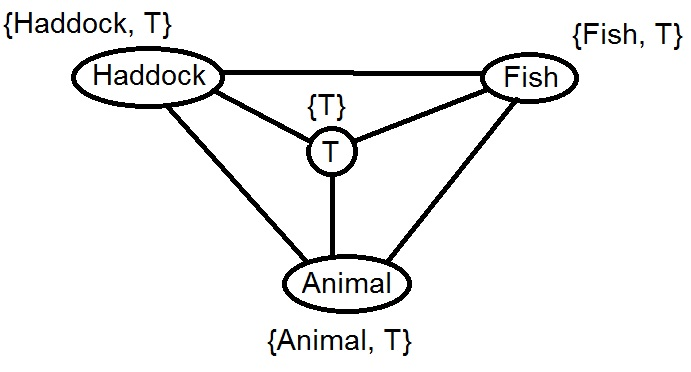
\includegraphics[scale=0.5]{Haddock-graph-with-T.jpg}}
\caption{Graph transformation of the TBox}
\label{hdk}
\end{figure}

\subsubsection{Complete the graph using completion rules}
The following three rules are then used to extend the sets $S$ and $R$:
\begin{itemize}
\item If $(A_1 \sqcap A_2 \sqsubseteq B) \in \mathcal{T}$ and $A_1, A_2 \in S(A)$ then add $B$ to $S(A)$
\item If $(A_1 \sqsubseteq \exists r.B) \in \mathcal{T}$ and $A_1 \in S(A)$ then add $r$ to $R(A, B)$
\item If $(\exists r.B_1 \sqsubseteq A_1) \in \mathcal{T}$ and $B_1 \in S(B), r \in S(A, B)$ then add $A_1$ to $S(A)$ 
\end{itemize}
If we apply the completion rules to $\mathcal{T}$, $S$ will become as follows:
\begin{itemize}
\item $S(Animal)= \lbrace Animal, \top \rbrace$
\item $S(Fish)= \lbrace Fish, \top, Animal \rbrace$
\item $S(Haddock) = \lbrace Haddock, \top, Fish, Animal \rbrace$
\end{itemize}
The new graph (after the completion rules are applied) can be visualised in Figure \ref{hdk-complete}. 

\begin{figure}
\centering
\fbox{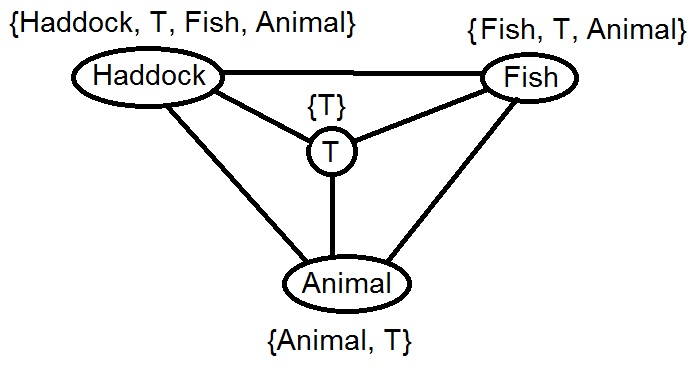
\includegraphics[scale=0.5]{Haddock-graph-with-T-complete.jpg}}
\caption{Completed graph of the TBox}
\label{hdk-complete}
\end{figure}

\subsubsection{Read off the subsumption relationships}
Now that the graph is complete, we can look at the sets $S$ and $R$ and determine whether the subsumption relationship in question holds or not. Since that subsumption relationship was $Haddock \sqsubseteq Animal$, we can look at $S(Haddock)$ and see if it contains $Animal$ or not, since the set $S(Haddock)$ contains all subsumers of $Haddock$. So, indeed, $Haddock \sqsubseteq Animal$ holds. This brief example hopefully shows a simple application of the subsumption algorithm of $\mathcal{EL}$. We didn't discuss the complexity of the algorithm in details, but it is enough to say it is polynomial in the size of the TBox. More details on the algorithm can be found in \cite{small} and \cite{new}.

Now that we had a quick introduction to the basic types of belief change and the framework of AGM, as well as the $\mathcal{EL}$ language and reasoning algorithm, we can start talking about the core of this study, which is kernel contraction. Throughout this study, we only consider DL knowledge bases represented in $\mathcal{EL}$. In the next chapter we look at an implementation of belief contraction using \textit{kernels} as introduced in \cite{zwei}. We will discuss some basic and general approaches as well as some more sophisticated ones. Then we will consider a language-specific approach to exploit the structure of $\mathcal{EL}$ and discuss heuristics that will provide more meaningful solutions. 

\chapter{Kernel contraction}
\label{kernel}
Belief contraction is the process of removing beliefs from belief sets. It can be done either by selecting one  of the largest subsets of the belief set that do not logically imply the abandoned belief, or by incising all the minimal subsets that logically imply that belief; by ``incising'' we mean removing a member from the set. The latter approach is the one we are going to focus on in this study. If a set $K$ of beliefs imply a belief $\alpha$, and $K$ is the minimal such set (no proper subset of $K$ implies $\alpha$), removing one element of $K$ will guarantee that it does not imply $\alpha$. Contraction is done here by finding all such minimum subsets and removing an element from each of them. We call such minimal sets \textit{kernels}. Kernels will be discussed in more details in the coming section. But we need to go over some definitions first.

Consider the following set:
\begin{center}
$ \lbrace a, a \rightarrow b, b, c \rbrace $
\end{center}
To contract the set by $b$, it is not enough to remove $b$ from the set. If we do so, we get:
\begin{center}
$ \lbrace a, a \rightarrow b, c \rbrace $
\end{center}
which still implies $b$. We need to prevent the resulting set of beliefs from implying $b$. The minimal subset that implies $b$ is 
\begin{center}
$ \lbrace a, a \rightarrow b \rbrace $
\end{center}
We call it a $b$-kernel. Since the kernel is a minimal subset that implies $b$, removing only one element of that kernel is enough to make it not imply $b$. The only other $b$-kernel of the original set is $\lbrace b \rbrace$; we can only break this kernel by removing $b$. Breaking the other kernel can be done either by removing $a$, or by removing $a \rightarrow b$. So the two possible resulting belief sets after contraction are:
\begin{center}
$ \lbrace a, c \rbrace $ and $ \lbrace a \rightarrow b, c \rbrace $
\end{center}
This is how kernel contraction works. Every $b$-kernel is one way to infer $b$. To contract $b$ every kernel should be broken by removing at least one belief. 


\section{What are kernels?}
Kernel contraction was introduced by Hansson\cite{kernel} as a variant of an older approach called ``safe contraction''\cite{safe}. In both approaches, contracting a knowledge base \textbf{K} by $\alpha$ is done by discarding beliefs that contribute to make \textbf{K} imply $\alpha$. Beliefs that contribute to make \textbf{K} imply $\alpha$ are members of some $\alpha$-kernels of \textbf{K}, and all members of every $\alpha$-kernel contribute to make \textbf{K} imply $\alpha$. In the previous example, there were two $b$-kernels: $\lbrace b \rbrace$ and $\lbrace a, a \rightarrow b \rbrace$. We need to remove at least one element from each kernel to contract the original set by $b$. We refer to the set of $\alpha$-kernels of \textbf{K} by $\textbf{K} \perp \alpha$.
\begin{defn}(Kernel Set)
According to \cite{hansson}, for a belief set \textbf{K} and a belief $\alpha$, $\textbf{K} \perp \alpha$ is a set such that $X \in \textbf{K} \perp \alpha$ if and only if:
\begin{enumerate}
\item $X \subseteq \textbf{K}$,
\item $X \vdash \alpha$, and
\item if $Y \subset X$ then $Y \nvdash \alpha$.
\end{enumerate}
$\textbf{K} \perp \alpha$ is a kernel set that contains all $\alpha$-kernels of \textbf{K}.
\end{defn}
Kernels are the smallest subsets of the knowledge base that imply a specific belief. Therefore, in order to give up that belief, every one of those kernels needs to be incised. If those kernels are not ``minimal'', they might contain some beliefs that do not contribute to make the kernel imply that specific belief. For example, in $\lbrace \alpha, \beta \rbrace$, $\beta$ is a belief that does not contribute to make the set imply $\alpha$. In that case, removing $\beta$ only would not help in giving up $\alpha$. 

So, because of the minimality of the kernels, every belief in the kernel is significant to implying the belief that we want to give up ($\alpha$). And that's why removing one belief from a kernel is sufficient to make that kernel not imply $\alpha$. So, we use a function that cuts every kernel in the kernel set. We call such function an \textit{incision function}; it takes a set of kernels and removes an element from each kernel. 

The incision function is defined in \cite{hansson} as follows:
\begin{defn}(Incision function)
An incision function $\sigma$ is a function such that for all beliefs $\alpha$:
\begin{enumerate}
\item $\sigma (A \perp \alpha) \subseteq \bigcup (A \perp \alpha)$
\item If $\phi \neq X \in A \perp \alpha$, then $X \cap \sigma (A \perp \alpha) \neq \phi$
\end{enumerate}
\end{defn}
Contraction is done by removing the beliefs that are selected by the incision function from the original knowledge base. Contraction $\approx_\sigma$ using the incision function $\sigma$ can be defined as:
\begin{defn}\cite{hansson} (Contraction)
\begin{center}
$A \approx_\sigma \alpha = A \smallsetminus \sigma (A \perp \alpha)$
\end{center}
\end{defn}


\section{Computing kernels}
Kernel contraction is about contracting knowledge bases using kernels. Kernels are the minimal subsets of the knowledge base that imply a certain consequence. The incision function can perform the contraction by cutting through all kernels of a specific belief. So, the first step in contraction is computing all kernels that imply the belief that needs to be removed. For that purpose, we use the pinpointing algorithm introduced in \cite{pin}.

To show how the algorithm works, we use the example introduced in \cite{pin}. Given an $\mathcal{EL}$ $TBox$ $\mathcal{T}$ consisting of the following four GCI axioms:
\begin{center}
$\mathcal{T} = \lbrace ax_1: A \sqsubseteq \exists{r}.A$, \hspace{7pt}  $ax_2: A \sqsubseteq Y$,  \hspace{7pt} $ax_3: \exists{r}.Y \sqsubseteq B$, \hspace{7pt} $ax_4: Y \sqsubseteq B \rbrace$,
\end{center}
we can see that $A \sqsubseteq B$ holds according to $\mathcal{T}$, i.e. $A \sqsubseteq_{\mathcal{T}} B$. Let: 
\begin{center} 
$\alpha = A \sqsubseteq B$.
\end{center}
According to the definition of kernel sets:
\begin{center}
$\mathcal{T} \perp \alpha = \lbrace \lbrace ax_2, ax_4 \rbrace, \lbrace ax_1, ax_2, ax_3 \rbrace \rbrace$
\end{center}
The algorithm introduced in \cite{pin} computes all kernels using a modified version of the $\mathcal{EL}$ subsumption algorithm. It works by finding a monotone boolean formula called \textit{``pinpointing formula''}. The propositions of the pinpointing formula are GCIs of the $TBox$, and a propositional \textit{valuation} represents the kernels. In that sense, a valuation is a set of propositional variables that satisfy the formula, and these variables are the GCIs that constitute a kernel. So, by finding all valuations of the pinpointing formula we can get all kernels.

In the worst case, this approach takes exponential time (w.r.t the size of the $TBox$) to find all kernels. This is the case when there are exponentially many kernels. However, \cite{pin} also gives a polynomial-time algorithm that computes only one kernel. Because it is not part of the scope of this study, we are not going to discuss and analyze details of the pinpointing algorithm. All that matters is the worst-case time complexity, as it will affect the complexity of the kernel contraction algorithm that uses it.


\section{Previous work}
We use the pinpointing algorithm to get the set of all kernels. We then need to remove one element from each kernel to perform contraction. This is the role of the incision function; it picks an element from each kernel so that it cuts through all kernels.
In this section, we look at some of the incision function implementations discussed in \cite{zwei}. The goal of this study is to continue the work started in \cite{zwei}, and to revise some of what has already been done. 

Given an $\mathcal{EL}$ $TBox$ $\mathcal{T}$ and a belief $\alpha$, ($\mathcal{T} \perp \alpha$) is the set of $\alpha$-kernels. The main contraction algorithm is shown in Algorithm \ref{MainAlgorithm}.

\begin{algorithm}
\caption{Contraction algorithm}
\label{MainAlgorithm}
\begin{algorithmic}[1]
\Procedure{contract}{$ \mathcal{T} $, A}
\State kernelset = \Call{pinpoint}{$ \mathcal{T} $, A}
\State giveUpSet = \Call{cut}{kernelset}
\State $\mathcal{T}$ = $\mathcal{T}$ / giveUpSet
\EndProcedure
\end{algorithmic}
\end{algorithm}

``kernelset'' refers to ($\mathcal{T} \perp \alpha$), and \textit{giveUpSet} is the set of beliefs selected by the incision function (CUT) to be removed. The algorithm is straightforward. It works by generating the set of kernels using the pinpoint formula as discussed in the previous section. Then it calls the incision function that picks up beliefs from every kernel, ensuring that it cuts all kernels. The beliefs are then removed from the knowledge base, i.e. from the $TBox$.

This general approach can be used with different incision functions. The call to the CUT function can be replaced with a call to another implementation of the incision function. The first implementation is the most straightforward one, where it removes a random belief from every kernel. This is given in Algorithm \ref{RandomAlgorithm}.

\begin{algorithm}
\caption{Random removal}
\label{RandomAlgorithm}
\begin{algorithmic}[1]
\Function{RandomRemove}{kernelset}
\State giveUpSet = $\lbrace \rbrace$
\For{$kernel \in kernelset$} 
\State choose a random belief $\alpha$ from $kernel$
\State giveUpSet = giveUpSet $\cup$ $\lbrace \alpha \rbrace$
\EndFor \State
\Return giveUpSet
\EndFunction
\end{algorithmic}
\end{algorithm}

The time complexity of RandomRemove function is polynomial: $O(m)$, where $m$ is the number of kernels (size of the kernelset), assuming that the random selection takes constant time. However, this is clearly not a good algorithm. In this example:
\begin{center}
kernelset = $\lbrace \lbrace a, c \rbrace, \lbrace b, c \rbrace \rbrace$, 
\end{center}
one of the possible outcomes of the RandomRemove algorithm is:
\begin{center}
\textit{giveUpSet} = $\lbrace c, b \rbrace$
\end{center}
which unnecessarily removes $b$. This could happen when the algorithm selects $c$ from the first kernel and $b$ from the second kernel. This solution:
\begin{center}
\textit{giveUpSet} = $\lbrace c \rbrace$
\end{center}
seems more concise and removes less beliefs. The second solution could be obtained if the algorithm is smart enough to check if the second kernel has already been incised. 

The next algorithm (Algorithm \ref{RandomExclusionAlgorithm}) does this. It goes over all kernels, and randomly selects a formula from every kernel to be removed. Every time it selects a belief, it marks all kernels that contain that belief so that they are not considered for belief removal in the following iterations. 

\begin{algorithm}
\caption{Random removal with exclusion}
\label{RandomExclusionAlgorithm}
\begin{algorithmic}[1]
\Function{RandomRemoveAndExclude}{kernelset}
\State giveUpSet = $\lbrace \rbrace$
\For{i=0 to size(kernelset)-1} 
\State kernelset[i].valid = true
\EndFor \State
\For{i=0 to size(kernelset)-1}
\If{kernelset[i].valid == true}
\State choose a random belief $\alpha$ from kernelset[i]
\State giveUpSet = giveUpSet $\cup$ $\lbrace \alpha \rbrace$
\For{j=i to size(kernelset)-1}
\If{kernelset[j].contains($\alpha$)}
\State kernelset[j].valid = false
\EndIf
\EndFor
\EndIf
\EndFor \State
\Return giveUpSet
\EndFunction
\end{algorithmic}
\end{algorithm}

Algorithm \ref{RandomExclusionAlgorithm} has a worst-case time complexity of $O(n^2)$, where $n$ is the size of the kernel set. This is because the second main loop has another nested loop inside it, and neither of them takes more than $n$ steps to finish. 

\section{Minimal change}
According to the information economy principal (minimality), in every change of the epistemic state, loss of information should be minimum\cite{econ}. This means that a system should choose an epistemic change outcome that minimizes loss of information. To satisfy the requirement of the minimum change we need an algorithm that removes the least number of GCIs while hitting all the kernels; but the kernels are nothing but sets of beliefs (GCIs). Luckily, this is exactly the \textit{minimal hitting set problem}, which already has some relatively efficient algorithms that we can use here. 

\subsection{Hitting set approach}
The minimal hitting set problem is defined as follows:
\begin{defn}\cite{hit}
Given a set $S=\{s_{1}, s_{2}, ..., s_{n}\}$ of $n$ non-empty sets, a minimal hitting set $d$ is a set such that:
\begin{center}
$\forall_{s_{i} \in S} [ s_{i} \cap d \neq \emptyset] \wedge \nexists_{d' \subset d}[\forall_{s_{i} \in S} (s_{i} \cap d' \neq \emptyset) ]$
\end{center}
\end{defn}

Thus, $d$ is a minimal hitting set if and only if it contains at least an element from every set, and no proper subset of it is a hitting set. In the context of kernel contraction in $\mathcal{EL}$, we can define the minimal hitting set contraction as:
\begin{defn}(Minimal hitting set contraction)
Given a kernelset $K=\{k_{1}, k_{2}, ..., k_{n}\}$ of $n$ kernels, a minimal hitting set $giveUpSet \subset K$ is a set such that:
\begin{center}
$\forall_{k_{i} \in K} [ k_{i} \cap giveUpSet \neq \emptyset] \wedge \nexists_{giveUpSet' \subset giveUpSet}[\forall_{k_{i} \in K} (k_{i} \cap giveUpSet' \neq \emptyset) ]$
\end{center}
\end{defn}

Since kernels are subsets of the $TBox$, and our goal to find a $giveUpSet$ that hits all kernels, we can use approaches to the minimal hitting set problem to solve it. There are good approximation algorithms, such as the one introduced in \cite{hit}, for the minimal hitting set problem, that are feasible in terms of running time. 

The notion of \textit{minimality} can be interpreted in terms of set-containment or cardinality. We call a hitting set minimal in terms of caridnality if there is no smaller-sized set that is a hitting set. However, the interpretation we use here is minimality accoring to set-containment; this means a minimal hitting set is a hitting set that has no proper subset that is a hitting set. So there might exist different minimal hitting sets with different cardinalities, but none of them is subsumed by a proper subset that is a hitting set\cite{hit}. But our goal was to satisfy the information economy principal by removing hitting sets with minimum cardinality. 

For that reason, after getting all minimum hitting sets, we need to consider only the ones that are smallest in size. For the kernel set:
\begin{center}
$kernelset = \lbrace \lbrace a, b \rbrace , \lbrace a, c \rbrace \rbrace$,
\end{center}
there are two minimal hitting sets:
\begin{center}
$\lbrace a \rbrace$ \hspace{1cm} and \hspace{1cm} $\lbrace b, c \rbrace$
\end{center}
and they are of different sizes. The following step then is to determine that the smallest of them should be selected for contraction, which is $\lbrace a \rbrace$.

We can now use one of the minimal hitting set algorithms combined with the cardinality selection step to implement contraction for a $TBox$, by implementing the minimal incision function that adopts them, to achieve minimum change (which we can call then, a \textit{minimal incision function}). We are not going to implement such a function in this study, but for now, we will assume that there is a function:
\begin{verbatim}
 min-hit-CUT(kernelSet)
\end{verbatim}
that takes a set of kernels, and returns a minimal hitting set (minimal in both set-containment and cardinality) of sentences to give up. We can use this function, as if it is implemented, and may implement it in some future work.

\subsection{Graph approach}
Now, we introduce another technique for kernel contraction in $\mathcal{EL}$ that is based on graphs. The reason why following graph approach is useful in solving contraction problem is that we are performing contraction of $TBoxes$, and they have an implicit graph-like hierarchy. 

An $\mathcal{EL}$ $Tbox$ consists of GCIs (we can transform all definition formulas to GCIs), that can be seen as nodes and edges. A GCI can be thought of as a directed edge between two nodes representing concepts on the two sides of the subsumption symbol ($\sqsubseteq$). So reasoning with $TBoxes$ is similar to reasoning with directed graphs. We can reduce $TBox$ reasoning problems to graph problems and use graph algorithms to solve them. The subsumption relationship that forms a $TBox$ seem to have an intuitive interpretation as a directed graph; and that's why we might use the word ``subsumption hierarchy'' later in this study to denote the relationship between concepts in the $TBox$.

The $\mathcal{EL}$ subsumption algorithm described in \cite{small} uses a graph approach, perhaps because it is intuitive to think of $TBoxes$ as graphs. A lot of work has been done in the area of Graph Theory, which makes it easy to use the already existing algorithms to solve some graph problems. Also, graphs are easy to imagine and work with. 

Our goal is to reduce the kernel contraction problem to a graph problem, and, using some efficient graph algorithms to perform kernel contraction. The algorithm we build here starts by transforming the $TBox$ into a graph. Then, it generates all kernels by finding all paths that imply the formula we are contracting. After that, it removes one formula from each kernel by removing an edge from each path, since paths here represent kernels (this will all be explained shortly). Finally it transforms the graph back into a $TBox$. 

We will start by describing the algorithm in details, and then explain each of its main steps. 

\subsubsection{Main algorithm}
%Every GCI of the form $C \sqsubseteq D \sqcap E$ can be decomposed into two GCIs: $C \sqsubseteq D$ and $C \sqsubseteq E$, where $C$, $D$ and $E$ are arbitrary concept expressions. 
Given an $\mathcal{EL}$ $TBox$ $T$, and a GCI $\mathbb{A}$ (where $\mathbb{A}$ is in the form of $C \sqsubseteq D$, such that $C$ and $D$ are arbitrary concept expressions), we contract $\mathcal{T}$ by $A$ using Algorithm \ref{GraphContract}:


\begin{algorithm}
\caption{Contraction using graph approach}
\label{GraphContract}
\begin{algorithmic}[1]
\Function {graphContract}{$ \mathcal{T} $, $\mathbb{A}$}
\State complete($ \mathcal{T} $)
\State graph = transform($ \mathcal{T} $)
\State C = $arg_{left}(\mathbb{A})$ $//$ gets the concept expression on the left side of the GCI
\State D = $arg_{right}(\mathbb{A})$ $//$ gets the right-side concept expression
\State paths = getPaths(graph, C, D)
\State cutPaths(graph, paths)
\State $ \mathcal{T} $ = de-transform(graph)
\EndFunction
\end{algorithmic}
\end{algorithm}

The complete function in step 2 uses the $\mathcal{EL}$ subsumption algorithm to compute all subsumptions of $\mathcal{T}$. All the subsumptions computed are added to $\mathcal{T}$. The subsumption algorithm proceeds in four steps:\cite{new}
\begin{enumerate}
\item Normalize the $TBox$.
\item Translate the normalized $TBox$ into a graph.
\item Complete the graph using completion rules.
\item Read off the subsumption relationship from the normalized graph.
\end{enumerate}
The algorithm is explained in full details in \cite{new}. We now need to explain the transformation of the $TBox$ $\mathcal{T}$ into a graph.

\subsubsection{Transforming the $TBox$ into a graph}
Assuming the $TBox$ $\mathcal{T}$ contains GCIs of the form $C \sqsubseteq D$ (where $D$ is an arbitrary concept, and $C$ is a concept expression of the form $c_1 \sqcap ... \sqcap c_n$ such that $n \geq 1$) , we construct a graph $graph=(V, E)$, where $V$ is a set of nodes and $E$ is a set of directed edges. Starting with an empty $V$ and $E$, for every GCI $C \sqsubseteq D$, add $C$ and $D$ to $V$, and add $(C, D)$ to $E$. This way every $v \in V$ represents a concept expression, and every pair $(C, D) \in E$ represents the subsumption relation $C \sqsubseteq D$.

\begin{algorithm}
\caption{Transforming a $TBox$ to a graph}
\label{Transformation}
\begin{algorithmic}[1]
\Function {transform}{$ \mathcal{T} $}
\State result = new Graph(V, E)
\For{every $C \sqsubseteq D$ in $ \mathcal{T} $}
\State $V = V \cup \{C, D\}$
\State $E = E \cup \{(C, D)\}$
\EndFor
\State \Return result
\EndFunction
\end{algorithmic}
\end{algorithm}

\subsubsection{Transformation analysis}
It is worth mentioning that even though subsumption can be decided in polynomial time with respect to the size of the $TBox$ (using the algorithm in \cite{small}), computing all subsumptions can be exponential in the number of concepts. For example, with:
\begin{center} 
$\mathcal{T} = \{Human \sqsubseteq Mammal, Mammal \sqsubseteq Animal\}$, 
\end{center}
the new $\mathcal{T}$ after adding all subsumptions would be: 
\begin{center}
$\{Human \sqsubseteq Human$, $Human \sqsubseteq Mammal$, $Human \sqsubseteq Animal$, $Mammal \sqsubseteq Mammal$, $Mammal \sqsubseteq Animal$, $Animal \sqsubseteq Animal\}$. 
\end{center}
The new $TBox$ contains a lot of unneeded GCIs. This can be avoided by adding a small step to the subsumption algorithm in \cite{small}, such that after completing the subsumption graph using the completion rules, we can remove all subsumptions of the form $X \sqsubseteq X$ (e.g. $Human \sqsubseteq Human$); also we need to remove all subsumptions $C \sqsubseteq D$ if $C \sqsubseteq X$ and $X \sqsubseteq D$ (e.g. exclude $Human \sqsubseteq Animal$ if $Human \sqsubseteq Mammal$, and $Mammal \sqsubseteq Animal$ are in the $TBox$) are already there.

Now we have a graph $graph$ that represents the $TBox$ $\mathcal{T}$. The next step is to compute the paths (using getPaths() function) from $C$ to $D$ (where $C$ and $D$ are graph nodes) using depth-first search. Obviously, computing the paths using depth-first search can take polynomial time. For simplicity, we assume the $TBox$ is acyclic. This means we don't allow the following situation:
\begin{center}
$\lbrace C \sqsubseteq D , D \sqsubseteq E , E \sqsubseteq C \rbrace$.
\end{center}
Thus, the graph must be acyclic too. The algorithm can still be generalized to account for cycles. Computing all paths can be done as in Algorithm \ref{GetPaths}.

\begin{algorithm}
\caption{Computing all paths between two nodes}
\label{GetPaths}
\begin{algorithmic}[1]
\Function {getPaths}{graph, C, D}
\State result = $\{\}$
\State Stack path = new empty Stack
\State computeAllPaths(graph, C, D, path, result)
\State \Return result
\EndFunction
\end{algorithmic}

\begin{algorithmic}[1]
\Function {computeAllPaths}{graph, C, D, path, paths}
\State graph = (V, E)
\For{every $(C, X) \in E$}
\If{X = D}
\State Stack temp = new empty Stack
\State temp.pushAll(path)  // adds all edges without changing path
\State temp.push($(C, X)$)
\State $paths = paths \cup \{temp\}$  // adding the path to the list of paths
\Else
\State path.push($(C, X)$)
\State computeAllPaths(graph, C, X, path, paths)
\State path.pop()
\EndIf
\EndFor
\EndFunction
\end{algorithmic}
\end{algorithm}

This can also be done if the graph contains cycles. It would require using a more complicated algorithm that keeps track of the number of edges and the nodes visited during execution. Finding paths in cyclic graphs in explained in details in \cite{alg}.

\subsubsection{Graph kernel contraction}
The function cutPath is the contraction function. Every path from $C$ to $D$ is actually a subsumption path that entails $C \sqsubseteq D$. Removing an edge from such path would break the subsumption between $C$ and $D$ through this path. So, in order to contract $C \sqsubseteq D$ it is enough to remove one edge from each of the paths from $C$ to $D$; as each path represents a \textit{kernel} of $C \sqsubseteq D$ and breaking them is sufficient to give up the subsumption. 

So, a simple and very easy implementation (though inefficient) for the contraction function is to go over the set of paths, and remove a random edge from every path. Suppose that the graph in Figure \ref{ex1} is interpreted as C is the most specific concept that is subsumed by A ($C \sqsubseteq A$), and as we climb the graph up, the concepts get more general. Here there are four C-D paths: (C, X, Z, A, E, D), (C, X, Z, A, F, D), (C, Y, Z, A, E, D), and (C, Y, Z, A, F, D). A function that removes random edges from each path might remove (C, X), (Y, Z), (E, D), and (F, D), which will actually remove the subsumption between C and D. However, it would be better (in terms of minimal change) to remove only (Z, A), which will also guarantee that subsumption between C and D is removed.

\begin{figure}
\centering
\fbox{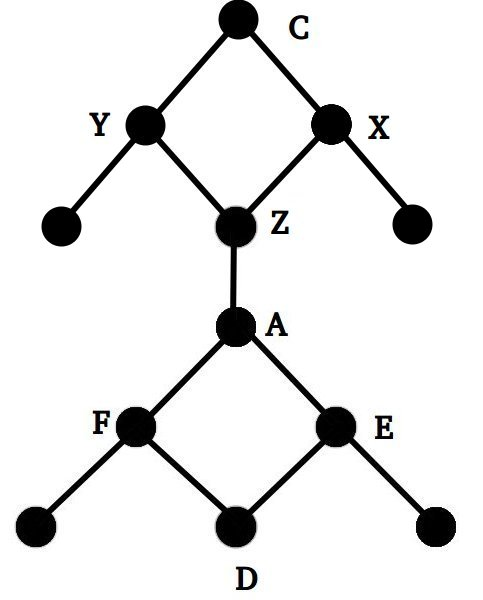
\includegraphics[scale=0.5]{example1.jpg}}
\caption{Four different paths between C and D, that share one edge.}
\label{ex1}
\end{figure}

Sometimes we prefer to remove GCIs that involve most specific concepts during contraction (this will be discussed in the coming chapter). To contract such GCIs, we can just remove, from each $C-D$ path, the edges going into $C$. In Figure \ref{ex1}, it would mean removing two edges: (C, X) and (C, Y). But removing such edges does not guarantee the minimum change. So we might end up having to choose which strategy is more preferred: minimal change or change with most specific concepts. The minimal hitting set approach that was mentioned earlier might not always satisfy specificity. So the user might have to choose which one to apply first, and which one to use as a tie breaker.

Removing the edges that involve nodes representing most specific concepts is straightforward; remove the edges that go into the most specific concept's node (C in our example). But it is not clear if one chooses to remove the least number of edges, instead, how this can be done. For this, we introduce an approach that uses the Minimum Cut algorithm to determine the minimum number of edges that need to be removed and identify them.

\subsubsection{Reduction to network flow problem}
As explained in \cite{alg}, the network flow problem is the problem of computing the maximum flow possible in a network (represented as a graph) by finding the minimum cut of the network. The input to the Ford-Fulkerson algorithm, that solves this problem, would be:
\begin{itemize}
\item A graph $G = (V, E)$.
\item A source $s \in V$.
\item A sink $t \in V$.
\item Capacity function $C:E \rightarrow \mathbb{N}$ representing the maximum capacity of each edge.
\end{itemize}

To contract $C \sqsubseteq D$ given the $TBox$ graph $G$, we choose $C$ to be the source, $D$ to be the sink, and we assume that the capacities of all edges are the same, equal to 1. The algorithm will find the maximum flow from $C$ to $D$, which is equal to the capacity of the minimum cut (the sum of capacities of the cut edges); we can then extract the edges that form that minimum cut and remove them.

The approach of removing the minimum cut edges of the graph is equivalent to the approach of removing the minimal hitting set formulas of the kernels. The minimal hitting set is the set containing the minimum number of elements that hit all sets, while the minimum cut of the graph is the minimum number of edges (since they all have the same capacity) that cover all paths from $C$ to $D$ (where edges represent GCIs of the $TBox$ and paths represent kernels.) So using the minimum cut approach should guarantee the minimum change for kernel contraction, as the minimal hitting set approach does.

Assuming we have a function ``Ford-Fulkerson(graph, s, t)'' that computes the maximum flow in the network (or graph) from source node ``s'' to a sink  ``t'' with edge-capacities ``1'', and returns the set of edges of the minimum cut, we can modify the contraction algorithm to adopt the minimum cut approach as in Algorithm \ref{GraphContract-modified}.

\begin{algorithm}
\caption{Another version of contraction algorithm}
\label{GraphContract-modified}
\begin{algorithmic}[1]
\Function {graphContractUsingMinCut}{$ \mathcal{T} $, $ \mathbb{A} $}
\State complete($ \mathcal{T} $)
\State graph = transform($ \mathcal{T} $)
\State C = $arg_{left}(\mathbb{A})$ $//arg_{left}$ gets the concept expression on the left side of the GCI
\State D = $arg_{right}(\mathbb{A})$ $//arg_{right}$ gets the right-side concept expression
\State min-cut = Ford-Fulkerson(graph, C, D)
\State remove min-cut edges from graph
\State $ \mathcal{T} $ = de-transform(graph)
\EndFunction
\end{algorithmic}
\end{algorithm}

For special cases such as contracting $C \sqsubseteq D1 \sqcap D2$, it is sufficient to contract $C \sqsubseteq D1$ first, and then contract $C \sqsubseteq D2$. But since the graph is already normalized (using complete() function), rules of the form $C \sqsubseteq D1 \sqcap D2$ are already broken down into two: $C \sqsubseteq D1$, and $C \sqsubseteq D2$. Therefore, the conjunction $\sqcap$ would only appear on the left hand side of a GCI in a normalized $TBox$ (e.g. $A1 \sqcap A2 \sqsubseteq B$). In that case, for contracting $A1 \sqcap A2 \sqsubseteq B$, there will be a node $A1 \sqcap A2$, which we will use as a source node; the sink would be the node representing $B$. 

As in \cite{alg}, the minimum cut algorithm runs in polynomial time. So using it in the contraction algorithm will not have a significant effect on the complexity of the main algorithm (will not elevate the complexity from being polynomial to being exponential). 

In some applications, the decision about which strategy to follow for choosing the edges to remove might vary depending on the situation. So the user can be asked in such case about which strategy to follow -- specificity or minimality. 

The last step of the algorithm is to transform the graph back to $\mathcal{EL}$. This can be done as follows: starting with an empty $TBox$ $\mathcal{T'}$, for every edge $(X, Y)$, add $X \sqsubseteq Y$ to $\mathcal{T'}$. The resulting $TBox$ would be the result of contracting $\mathcal{T}$ by $\mathbb{A}$. This is shown in Algorithm \ref{DeTransform}.

\begin{algorithm}
\caption{Transforming a graph back to a $TBox$}
\label{DeTransform}
\begin{algorithmic}[1]
\Function {de-transform}{graph}
\State result = $\{\}$
\State graph = (V, E)
\For{every $(X, Y) \in E$}
\State $result = result \cup \{X \sqsubseteq Y\}$
\EndFor
\State \Return result
\EndFunction
\end{algorithmic}
\end{algorithm}

Since the running time of every step of the contraction algorithm starting from ``transform($ \mathcal{T} $)'' until the last step is polynomial in the size of the $TBox$, the complexity of the algorithm will depend on the complexity of the first step (the complete() function). If building the subsumption hierarchy by generating all subsumptions of an $\mathcal{EL}$ $TBox$ can be done in polynomial time, then the contraction algorithm will in turn take polynomial time. But if generating all subsumptions takes exponential time, then the algorithm will take exponential running time as well.

\subsubsection{A Sample Run}
Suppose we have a TBox $\mathcal{T}$:
\begin{center}
$\mathcal{T} = \lbrace A \sqsubseteq B, B \sqsubseteq C \rbrace$
\end{center}
which implies $A \sqsubseteq C$. Trying to contract $\mathcal{T}$ by $A \sqsubseteq C$ using the network flow approach would work as follows:
\begin{enumerate}
\item complete($\mathcal{T}$). 
The TBox is already normalized. Translating it into a graph and applying the completion rules will introduce $A \sqsubseteq C$ and will be added explicitly to the TBox.
\item transform($\mathcal{T}$).
After transforming the TBox into a graph, it will look like the graph in Figure \ref{fig:abc-kb}.

\begin{figure}
\centering
\fbox{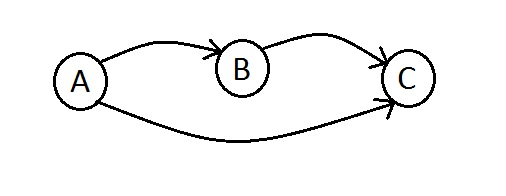
\includegraphics[scale=0.5]{abc-kb.jpg}}
\caption{Graph representing TBox $\mathcal{T} = \lbrace A \sqsubseteq B, B \sqsubseteq C, A \sqsubseteq C \rbrace $}
\label{fig:abc-kb}
\end{figure}

\item getPaths(graph, A, C) will get all paths between A and C. There are only two paths: A-B-C and A-C. 

\item Cutting the two paths A-B-C and A-C will be done by removing the edge between A and C, as well as one of the two edges A-B and B-C. So the resulting graph will only have one edge: A-B or B-C.

\item After transforming the graph again into a TBox, the result will be:
\begin{center}
$\mathcal{T} = \lbrace A \sqsubseteq B \rbrace$
\end{center}
or 
\begin{center}
$\mathcal{T} = \lbrace B \sqsubseteq C \rbrace$.
\end{center}

\end{enumerate}


\subsubsection{The limitations of the algorithm}
The previous example shows how the algorithm succeeds in finding the set of kernels by finding the paths from the source to the sink (where source and sink represent the two sides of the GCI that we need to remove). The example we will discuss now shows how the conjunction symbol ($\sqcap$) might introduces further complexity that the algorithm will not overcome. Given the TBox $\mathcal{T}$:
\begin{center}
$\mathcal{T} = \lbrace A \sqsubseteq B, A \sqsubseteq C \rbrace$
\end{center}
we can see that it entails
\begin{center}
$A \sqsubseteq B \sqcap C$.
\end{center}
If we want to contract the TBox by $A \sqsubseteq B \sqcap C$, we would look for its kernels and remove a statement from each. In this example we have only one kernel:
\begin{center}
$\lbrace A \sqsubseteq B, A \sqsubseteq C \rbrace$.
\end{center}
So removing one of the two GCIs is enough to give up $A \sqsubseteq B \sqcap C$. Contracting it using our graph approach works as follows:

\begin{enumerate}
\item complete($\mathcal{T}$). 
The TBox is already normalized. Translating it into a graph and applying the completion rules will introduce $A \sqsubseteq B \sqcap C$ and will be added explicitly to the TBox.
\item transform($\mathcal{T}$).
After transforming the TBox into a graph, it will look like the graph in Figure \ref{fig:abcbc-kb}.

\begin{figure}
\centering
\fbox{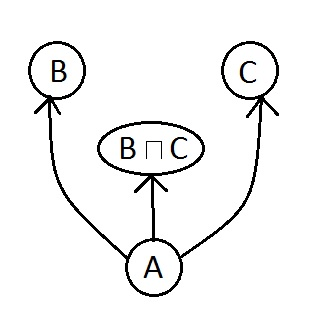
\includegraphics[scale=0.5]{abcbc-kb.jpg}}
\caption{Graph representing TBox $\mathcal{T} = \lbrace A \sqsubseteq B, A \sqsubseteq C, A \sqsubseteq B \sqcap C \rbrace $}
\label{fig:abcbc-kb}
\end{figure}

\item getPaths(graph, $A$, $B \sqcap C$) will get all paths between $A$ and $B \sqcap C$. There is only one such path, which is the edge between them. So cutting this edge would be the only possible outcome of the algorithm.
\end{enumerate}

This last step is where the algorithm fails. It finds only one of the kernels because it does not recognize that the two parallel edges from A to B and C actually form another kernel. This is because a kernel in our graph approach can only be represented as a path. The conjunction symbol $\sqcap$ has a different meaning, and is not analogous to the path notion. However, the algorithm worked with the previous example because the GCI we tried to remove was the result of applying the transitivity property of the subsumption symbol ($\sqsubseteq$) to two other GCIs and they together were represented by a path in the graph representation.

Similarly, we can argue that the algorithm also fails when the existential quantification symbol ($\exists$) is used. For example, the following TBox:
\begin{center}
$\mathcal{T} = \lbrace A \sqsubseteq \exists r.B, B \sqsubseteq C \rbrace$
\end{center}
implies the following expression:
\begin{center}
$A \sqsubseteq \exists r.C$
\end{center}
The graph approach will not get the kernels of that expression using the getPaths() function. So, it will also fail. But this is only because of the subsumption of $B$ by $C$, where $B$ is included in the role expression $\exists r.B$. If the existential quantification symbol is used without changing the symbols involved in the roles (such as $B$), the algorithm will work fine, as it will only be depending on the subsumption relations between concept expressions.

So it seems that the limitations of this algorithm are only due to the difference between the inference using paths between nodes and inference the introduces conjunction or existential quantification. However, the algorithm does not always fail when $\sqcap$ or $\exists$ is involved. In Figure \ref{fig:abc-kb}, if we replace B by (X $\sqcap$ Y), or by  ($\exists r.$B), the algorithm will succeed. That is because the nodes do not change after the inference; all that is added by the subsumption algorithm are new edges. 


\subsubsection{Analysis of the graph algorithm}
It is important to be able to measure the correctness of the solution we get by running the algorithm. The AGM framework provides a set of rationality postulates for contraction that we use for this purpose. Let's see whether the algorithm satisfies each of those postulates. 

\begin{description}
\item[(K $-$ 1)] For any sentence $A$ and any belief set $K$, $K^{-}_{A}$ is a belief set.
\end{description}
Since the algorithm only removes edges (or GCIs), the remaining set of edges still represent a set of GCIs, which is a belief set.
\begin{description}
\item[(K $-$ 2)] $K^{-}_{A} \subseteq K$. 
\end{description}
This is also satisfied as the new set is obtained by only removing GCIs.
\begin{description}
\item[(K $-$ 3)] If $A \notin K$, then $K^{-}_{A} = K$. 
\end{description}
If the algorithm is given a GCI that is not in the set, the source and sink nodes will not be in the graph. In this case, the minimum cut algorithm will not have any flow and will not remove any edges. So, the set will remain the same after contraction.
\begin{description}
\item[(K $-$ 4)] If not $\vdash A$, then $A \notin K^{-}_{A}$. 
\end{description}
If a GCI is given the algorithm, the remaining set after contraction will not contain this GCI, because the edge between both sides of the GCI will be removed. By having the edge removed, the transformation of the graph into a TBox will not create such GCI.
\begin{description}
\item[(K $-$ 5)] If $A \in K$, then $K \subseteq (K^{-}_{A})^{+}_{A}$.
\end{description}
This is called the recovery postulate. This is not satisfied by the algorithm. The reason for this is that if a GCI is contracted by the algorithm, this can sometimes involve removing some edges along the path from the source node to the sink node. Adding the GCI back to the new set will not trigger the introduction of those other edges that were removed.
\begin{description}
\item[(K $-$ 6)] If $\vdash A \leftrightarrow B$, then $K^{-}_{A} = K^{-}_{B}$.
\end{description}
This is trivially satisfied, because in $\mathcal{EL}$ two GCIs are equivalent if and only if they are exactly the same.
\begin{description}
\item[(K $-$ 7)] $K^{-}_{A} \cap K^{-}_{B} \subseteq K^{-}_{A \& B}$.
\end{description}
The algorithm contracts only one belief at a time. If we would like to contract something like $(A \& B)$, we would do it by either contracting $A$ or contracting $B$ (contracting $(A \& B)$ is the same as contracting one of them). And since contraction is monotonic (it only removes GCIs), the set resulting from contracting $A$ cannot be bigger than the original, and same with $B$. Thus, the intersection of both of them cannot be bigger than one of them (as no other GCIs were introduced).
\begin{description}
\item[(K $-$ 8)] If $A \notin K^{-}_{A \& B}$, then $K^{-}_{A \& B} \subseteq K^{-}_{A}$.
\end{description}
If $A$ is not present after contracting $(A \& B)$, it means that contraction of $(A \& B)$ was done by contracting $A$. In this case, the remaining set is the same for both contractions.

\subsection{How to generate kernels?}
So far, we have discussed two ways for generating all kernels:
\begin{enumerate}
\item Using the pinpointing algorithm.
\item Using the graph approach.
\end{enumerate}
Computing kernels using the graph approach finds all kernels by performing depth-first search on the graph representation of the TBox. It finds all kernels in $O(E)$, where $E$ is the number of edges in the graph (or the number of GCIs in the TBox). However, it only works with subsumptions that do not include the conjunction symbol ($\sqcap$). So, in cases where the conjunction is not used in the TBox, the graph approach will be at least as efficient as the pinpointing approach, if not better (the axiom pinpointing algorithm introduced in \cite{pin} finds one kernel in polynomial time).


\subsection{What incision function to use?}
If we care about selecting minimum number of beliefs to remove, then there are two incision approaches we discussed so far:
\begin{enumerate}
\item The minimum hitting set algorithm.
\item The minimum cut algorithm for the network flow problem.
\end{enumerate}
The minimum hitting set problem is NP-hard. However, the algorithm we discussed in this study is a relatively efficient approximation algorithm. However, in cases where the minimum cut approach can be used, the minimum cut algorithm is probably the best and most efficient. The algorithm works by finding the max flow possible through the network build from the TBox, and then uses it to find the minimum cut.

The Ford-Fulkerson maximum flow algorithm typically takes $O(E.C)$ steps to find the maximum flow, where $E$ is the number of edges and $C$ is the sum of all capacities. Since all edges in our approach has capacity 1, $C$ is equal to $E$. So the complexity of the algorithm is $O(E^2)$. After finding the maximum flow, we can find the minimum cut in $O(E)$. So the overall complexity of the algorithm is $O(E^2)$.

In other cases where the graph approach is not applicable, the minimum hitting set algorithm is a good candidate. In the next chapter, we will also give some techniques for implementing the incision function. Some of them might be even more suitable than the minimum hitting set approach, depending on the domain and the preferences of the user.


\chapter{Heuristics for contraction}
Considering algorithms that guarantee minimum change during contraction is not always enough to achieve optimal contraction. So far, we have considered minimal contraction by trying to find the smallest \textit{giveUpSet}. However, we haven't considered the significance of the subsumption hierarchy of $\mathcal{EL}$ in contracting a $TBox$. In this chapter, we look at heuristics that are motivated by the subsumption relationship between formulas. We will discuss ways of determining a preferred set of beliefs to be removed, based on the subsumption relationship of $\mathcal{EL}$ represented by the symbol $\sqsubseteq$. 

According to \textit{localization} and \textit{specificity} heuristics\footnote{These heuristics will be explained shortly.}, we can prefer to remove a certain set of beliefs to another, even if it is of bigger or equal size. We can say that it is ``semantically better'' to remove beliefs that are related than to remove unrelated beliefs; by ``semantically'' we mean according to the meaning of the language's logical connectives. Also, it is better to remove beliefs about specific concepts than general ones. These two selection heuristics, localization and specificity, can be used as tie-breakers when we have multiple \textit{giveUpSets} of the same size and we need to select only one. They can also be used on their own regardless of the size of the \textit{giveUpSets}.

Before discussing localization and specificity, there is another approach that is worth mentioning. That approach is the \textit{Greedy} approach that was introduced in \cite{zwei}. It does not account for the subsumption relationship between $\mathcal{EL}$ concepts (it is language independent). It only cares about the intersection between kernels. After explaining how it works, we will turn to the two language-dependent heuristics and see how they work.


\section{Greedy Contraction}
The greedy approach works by selecting the beliefs that appear in more kernels to be removed before those that appear in less kernels. At each step, the algorithm finds which belief appears the most in kernels and removes it, and then it forgets about those kernels (it does not consider those kernels that contain the removed belief for the following steps). This means that if a belief is selected for removal, all the kernels that contain it are already incised and no more beliefs need to be removed from these kernels.

\begin{algorithm}
\caption{Greedy Selection}
\label{GreedyAlgorithm}
\begin{algorithmic}[1]
\Function {GreedyContract}{$kernelset, beliefs$}
\State $initializeValidKernels(kernelset)$
\State $initializeBeliefOccurrences(beliefs)$
\State $computeOccurrences(kernelset, beliefs)$
\State \Return $selectMaxBeliefs($kernelset, beliefs$)$
\EndFunction
\end{algorithmic}
\end{algorithm}

\begin{algorithm}
\begin{algorithmic}[1]
\Function{initializeValidKernels}{$kernelset$}
\State $validKernels = 0$ $// global \: variable$
\For{$i = 1$ to $size(kernelset)$}
\State $validKernel[i] = 1$  $// global \: array$
\State $validKernels = validKernels + 1$
\EndFor
\EndFunction
\end{algorithmic}

\begin{algorithmic}[1]
\Function{initializeBeliefOccurrences}{$beliefs$}
\For{$i = 1$ to $size(beliefs)$}
\State $occurs[i] = 0$  $// global \: array$
\EndFor
\EndFunction
\end{algorithmic}

\begin{algorithmic}[1]
\Function{computeOccurrences}{$kernelset, beliefs$}
\For{$i=1$ to $size(beliefs)$}
\For{$j=1$ to $size(kernelset)$}
\If{$kernelset[j].contains(beliefs[i])$}
\State $occurs[i] = occurs[i] + 1$
\EndIf
\EndFor
\EndFor
\EndFunction
\end{algorithmic}

\begin{algorithmic}[1]
\Function{selectMaxBeliefs}{$kernelset, beliefs$}
\State $giveUpSet = \lbrace \rbrace$
\While{$validKernels > 0$}
\State $max = 0$
\State $maxIndex = 0$

\For{$i=1$ to $size(beliefs)$}
\If{$occurs[i]>max$}
\State $max = occurs[i]$
\State $maxIndex = i$
\EndIf
\EndFor

\For{$i=1$ to $size(kernelset)$}
\If{$kernelset[i].contains(beliefs[maxIndex])$}
\State $validKernel[i] = 0$
\State $validKernels = validKernels - 1$
\State updateOccurrences($kernelset[i], beliefs$)
\EndIf
\EndFor
\State $occurs[maxIndex] = 0$
\State $giveUpSet = giveUpSet \cup \lbrace beliefs[maxIndex] \rbrace$
\EndWhile
\State \Return $giveUpSet$
\EndFunction
\end{algorithmic}
\end{algorithm}

\begin{algorithm}
\begin{algorithmic}[1]
\Function{updateOccurrences}{$kernel, beliefs$}
\For{$i=1$ to $size(kernel)$}
\State $removeOccurances(beliefs, kernel[i])$
\EndFor
\EndFunction
\end{algorithmic}

\begin{algorithmic}[1]
\Function{removeOccurrences}{$beliefs, belief$}
\For{$i=1$ to $size(beliefs)$}
\If{$beliefs[i] == belief$}
\State $occurs[i] = occurs[i] - 1$
\EndIf
\EndFor
\EndFunction
\end{algorithmic}
\end{algorithm}

Algorithm \ref{GreedyAlgorithm} explains how the greedy approach for contraction works. Given a set of kernels and the set of all beliefs (the knowledge base), it proceeds as follows: it computes the number of occurrences of every belief in the kernels given, then it removes them one by one starting from the beliefs with maximum number of occurrences, until all kernels are incised. It does not actually remove the beliefs, but it collects them in the $giveUpSet$ that will be returned to the main contraction, which in turn will remove them from the knowledge base. So the greedy approach can be embedded in the main algorithm as a way to choosing the beliefs that need to be removed. 

The worst-case time complexity of the greedy algorithm is lower-bounded by the complexity of the ``while'' loop in the $selectMaxBeliefs()$ function. If the size of $beliefs$ is $m$, the size of $kernelset$ is $n$, and the size of the biggest $kernel$ is $k$, then the worst-case time complexity is $O(n^2 \cdot k \cdot m)$. This could be significantly enhanced by using more clever data structures to make the in-validation of the kernels (the step where we decrement the number of valid kernels and update the occurrences) faster. But this is not very important now, because the greedy algorithm does not add to the optimality we are targeting in this chapter. As said before, the greedy algorithm only targets the minimality.

The rest of the chapter will be dedicated to discussing other heuristics that aim at achieving more optimal results by exploiting the structure and hierarchy of the $\mathcal{EL}$ TBoxes.

\section{Localization}
Giving up beliefs about a certain concept means being in doubt of this concept. The more beliefs we remove, the more concepts we become in doubt of. This can lead us to consider removing beliefs about a certain concepts rather than beliefs about many different concepts. As discussed in \cite{zwei}, it is more efficient to remove beliefs that share concepts or roles in a TBox as it means being in doubt of less number of concepts.

This seems a reasonable approach as humans tend to deal with related beliefs than unrelated ones. If we try to revise our knowledge, we will probably find ourselves leaning towards focusing on beliefs that share common concepts. 

The following $\mathcal{EL}$ example:
\begin{center}
(1) $AspergillusFumigatus \sqsubseteq Multicellular $ \\
(2) $Multicellular \sqsubseteq NotBacteria$ \\
(3) $AspergillusFumigatus \sqsubseteq Eukaryotes$ \\
(4) $Eukaryotes \sqsubseteq NotBacteria$ 
\end{center}
implies:
\begin{center}
(5) $AspergillusFumigatus \sqsubseteq NotBacteria$,
\end{center}
and we can see that there are two (5)-kernels:
\begin{center}
\{1, 2\} and \{3, 4\}
\end{center}

So, to contract the knowledge base by (5), we need to remove a belief from each kernel. However, removing (1) and (4) seems unreasonable because it means that we are in doubt of our knowledge of $AspergillusFumigatus$, $Multicellular$ beings, $Eukaryotes$, and beings that are $NotBacteria$, while removing (1) and (3), on the other hand, makes us in doubt only of our knowledge of $AspergillusFumigatus$, $Multicellular$ beings, and $Eukaryotes$. Not only that, but removing (1) and (3) actually means that our knowledge of $AspergillusFumigatus$ is wrong; Our knowledge of $Multicellular$ beings and $Eukaryotes$ is not necessarily false. Same with removing (2) and (4), we suspect the soundness of our beliefs about beings that are $NotBacteria$.

Localization is implemented in \cite{zwei} using a graph-like approach. The algorithm operates by defining edge-like relationship between formulas and using graph connectivity and graph clustering rules to determine localized sets. 

\begin{defn}
For every two GCIs $\mathbb{X}$ and $\mathbb{Y}$, we say that there is an edge between them if they share a concept or role.
\end{defn}

After applying that, we will end up with a graph-like structure, where some GCIs of the knowledge base are connected by edges. The most basic path in a graph is an edge, but a path can be composed of more than one edge. Generally, a path is a sequence of edges.

\begin{defn}(Conncected GCIs)
Two GCIs $\mathbb{A}$ and $\mathbb{B}$ are connected if and only if there is a path from one of them to the other, i.e. if there is a sequence of edges and GCIs $Ae_1G_1e_2 ... G_{n-1}e_nB$, where $G_i$ is a GCI, $e_i$ is an edge, every triple $G_ie_{i+1}G_{i+1}$ means $G_i$ and $G_{i+1}$ are connected by an edge, and $n \geq 0$.
\end{defn}

So, in the last $\mathcal{EL}$ example, we can remove one of the following sets to contract (5):
\begin{itemize}
\item \{1, 3\} (a)
\item \{1, 4\}. (b)
\end{itemize}

There are more possible \textit{giveUpSets}, but (a) and (b) are sufficient to show how the definition of connected GCIs can be applied. 

For the set (a), there is an edge between (1) and (3) because they share the same concept \textit{AspergillusFumigatus}. So, according to the definition, (1) and (3) are connected.

For the set (b), there is no edge between (1) and (4) because they don't share any concept or role. So according to the definition, (1) and (4) are not connected.

\begin{defn}(Clusters)
A GCI $\mathbb{X}$ belongs to a cluster $\mathfrak{C}$ if and only if $\mathbb{X}$ is connected to every GCI in $\mathfrak{C}$.
\end{defn}

Thus, according to the definitions, the set (a) has only one cluster, as (1) and (3) are connected and belong to the same cluster. However, the set (b) has two clusters, because (1) and (4) are not connected in (b), so they belong to two different clusters.

The algorithm uses the notion of clusters to identify the best \textit{giveUpSet}. A GCI belong to a cluster if it shares concepts or roles with other GCIs in the \textit{giveUpSet}. If a \textit{giveUpSet} contains a lower number of clusters than another set, then it is better to remove it during contraction. This is because the more clusters there is in a set the more sparse the graph is, hence the less localized the contraction is. 

The algorithms works on each possible \textit{giveUpSet} separately. It builds the graph-like edges between formulas in the set according to the definitions we gave. It is important that the algorithm computes the connectivity in each set separately, because two formulas might have a path between them in one set but not the other; so they would be considered connected in a set and disconnected in the other. The algorithm then counts the number of clusters. It does that for all the sets, then chooses the set with least number of clusters to be removed.

\begin{algorithm}
\caption{Computing localized hit}
\label{LocalizeContraction}
\begin{algorithmic}[1]
\Function{getLocalizedHit}{giveUpSets}
\State $setWithLeastClusters = null$
\State $smallestNumber = \inf$
\For{$giveUpSet \in giveUpSets$}
\State $numOfClusters = getNumberOfClusters(giveUpSet)$
\If{$numOfClusters < smallestNumber$}
\State $setWithLeastClusters = giveUpSet$
\State $smallestNumber = numOfClusters$
\EndIf
\EndFor
\State \Return $setWithLeastClusters$
\EndFunction
\end{algorithmic}


\begin{algorithmic}[1]
\Function{getNumberOfClusters}{giveUpSet}
\For{$i=1$ to $size(giveUpSet)$}
\State $label[i]=i$
\EndFor
\For{$i=1$ to $size(giveUpSet)$}
\State $cluster[i]=0$
\EndFor
\For{$i=1$ to $size(giveUpSet)$}
\For{$j=i+1$ to $size(giveUpSet)$}
\If{giveUpSet[i] and giveUpSet[j] are connected}
\State $label[j] = label[i]$
\EndIf
\EndFor
\EndFor
\For{$i=1$ to $size(giveUpSet)$}
\State $cluster[label[i]]=1$
\EndFor
\For{$i=1$ to $size(giveUpSet)$}
\State $numberOfClusters = numberOfClusters + cluster[i]$
\EndFor 
\State \Return $numberOfClusters$
\EndFunction
\end{algorithmic}
\end{algorithm}

Algorithm \ref{LocalizeContraction} selects the giveUpSet with least number of clusters by first computing the number of clusters in each giveUpSet and then choosing the one with the smallest number.

\section{Specificity}

The subsumption hierarchy enforced by the subsumption relation in $\mathcal{EL}$ categorizes beliefs (or GCIs) into different levels of generality and specificity. Consider the kernel:% in Figure \ref{fig:AnimalKernel},
\begin{figure}[h]
\begin{center}
$Lion \sqsubseteq Mammal$\\
$Mammal \sqsubseteq Vertebrate$\\
$Vertebrate \sqsubseteq Animal$
\end{center}
\caption{Simple Animal kernel}
\label{fig:AnimalKernel}
\end{figure}

which implicitly entails
\begin{center}
$Lion \sqsubseteq Animal$
\end{center}
And suppose we would like to contract the $TBox$ by $Lion \sqsubseteq Animal$. We have three options: we can remove $Lion \sqsubseteq Mammal$, $Mammal \sqsubseteq Vertebrate$, or $Vertebrate \sqsubseteq Animal$. Removing any of the three GCIs would guarantee minimum change. However removing $Lion \sqsubseteq Mammal$ sounds much more reasonable than removing $Vertebrate \sqsubseteq Animal$: $Lion \sqsubseteq Mammal$ involves concepts that are more specific than the ones involved in $Vertebrate \sqsubseteq Animal$. Removing $Vertebrate \sqsubseteq Animal$ may affect more concepts in the subsumption hierarchy (in worst case) than those affected by removing $Lion \sqsubseteq Mammal$. 

So, it is preferable to remove GCIs that involve specific concepts rather than removing GCIs that involve more general ones. To account for specificity, we assign a label to each of the concepts representing its level in the subsumption hierarchy, where levels increase with generality. And during contraction, we consider contracting GCIs that involve concepts at lower level before considering GCIs that involve concepts at higher level.

The approach we follow in this study for adopting the preference of removing sentences that contain more specific concepts is by assigning weights to every GCI that reflects its generality, then we select the kernels with minimal overall weight. Every GCI gets a numeric weight depending on the level of generality of the concepts involved in it (depending on their position in the subsumption graph). A GCI $A \sqsubseteq B$ gets weight `0' if $A$ has no children, i.e. if there is no rule of the form $X \sqsubseteq A$, where $X$ is an arbitrary concept; and the GCI involving its parent will have weight `1' in that case. So the weight somehow represents the level in the subsumption graph, starting from level `0' at the trees' roots. For simplicity, we assume that the $TBox$ is acyclic -- so we avoid the problems that will be caused by loops.


Similar to the hierarchy of the subsumption graph of an $\mathcal{EL}$ TBox, we give a definition to \textit{parent} and \textit{child} concepts as follows:
\begin{defn}
\label{defn:Parent-Child}
For the GCI $A \sqsubseteq B$:
\begin{itemize}
\item $A$ is a \textit{child} concept relative to $B$, and
\item $B$ is a \textit{parent} concept relative to $A$.\\
\end{itemize}
\end{defn}

So by looking again at Figure \ref{fig:AnimalKernel}, we can now say that:
\begin{itemize}
\item Mammal is a \textit{parent} of Lion, and Lion is a \textit{child} of Mammal
\item Vertebrate is a \textit{parent} of Mammal, and Mammal is a \textit{child} of Vertebrate
\item Animal is a \textit{parent} of Vertebrate, and Vertebrate is a \textit{child} of Animal
\item Animal is the most \textit{general} concept, i.e. Animal subsumes all other concepts
\item Lion is the most \textit{specific} concept (least \textit{general}), i.e. it is subsumed by all other concepts
\item $Lion \sqsubseteq Mammal$ has weight = 0
\item $Mammal \sqsubseteq Vertebrate$ has weight = 1
\item $Vertebrate \sqsubseteq Animal$ has weight = 2
\end{itemize}

The algorithm we introduce now removes kernels that contain GCIs involving most specific concepts by first computing the weights of every kernel based on the weights of the GCIs inside it. Following Definition \ref{defn:Parent-Child}, we start the algorithm by building the $children$ labels for all the concepts in the $TBox$ that we will use to assign weights to the GCIs. Given a $TBox$ $T$, the algorithm proceeds as in Algorithm \ref{GraphBuild}.

\begin{algorithm}
\caption{Building the children graph}
\label{GraphBuild}
\begin{algorithmic}[1]
\Function{graphBuild}{T}
\State $children(X) = \emptyset$, for every concept X in T 
\For{every $A \sqsubseteq B \in T$}
\State $children(B) = children(B) \cup \{ A \}$
\EndFor
\EndFunction
\end{algorithmic}
\end{algorithm}

Now we have a graph composed of concepts and their $children$ relation; the nodes are concepts and the edges are the child-parent relationship between them. The roots are now concepts with no parents, and the leaves are concepts with no children. The GCIs involving leaves are assigned weight `0' and it increases by `1' every step towards the roots. So, the roots are most general concepts, and the leaves are most specific. If a GCI contains concepts $\alpha \sqsubseteq \beta$, where $\alpha$ has no parents and $\beta$ has no children, then it gets weight `0' according to Algorithm \ref{AssignWeights}.

\begin{algorithm}
\caption{Assigning Weights}
\label{AssignWeights}
\begin{algorithmic}[1]
\Function {assignWeights}{T}
\For{every $A \sqsubseteq B \in T$}
\State $weight(A \sqsubseteq B) = GetWeight(A \sqsubseteq B)$
\EndFor
\EndFunction
\end{algorithmic}

\begin{algorithmic}[1]
\Function {getWeight}{$X \sqsubseteq Y$}
\If{$weight(X \sqsubseteq Y) \neq NULL$}
\State
\Return $weight(X \sqsubseteq Y)$
\EndIf
\If{$children(X) = \emptyset$}
\State
\Return 0
\Else
\State
\Return $1 + GetMaxWeight(X)$
\EndIf
\EndFunction
\end{algorithmic}

\begin{algorithmic}[1]
\Function {getMaxWeight}{X}
\State max = -- 1
\For{every Z in children(X)}
\State w = GetWeight($Z \sqsubseteq X$)
\If{ w $>$ max}
\State max = w
\EndIf
\EndFor
\State
\Return max
\EndFunction
\end{algorithmic}
\end{algorithm}

Now we have every GCI in T assigned a weight relative to its level of generality. So, in every kernel we have a preference level of what to give up. Based on the weights, we will choose the sentences with less weight over the ones with more weight to remove. This preference can be used as a tie-breaker after we apply the minimal hitting set algorithm and end up with more than one minimal set. If we arrive at two minimal hitting sets for the kernels, we can compute the overall weight of each of the hitting sets and remove the sentences in the one with lower weight. This is shown in Algorithm \ref{RemoveSpecific}. It uses the min-hit-CUT algorithm that gets the minimum hitting sets given a kernel set. There could be more than one minimum hitting set.

\begin{algorithm}
\caption{Removing specific hitting set}
\label{RemoveSpecific}
\begin{algorithmic}[1]
\Function {getMostSpecificHit}{kernelset}
\State min-hit-sets = min-hit-CUT(kernelSet)
\State $min = \infty$
\State hit = NULL
\State w(s) = 0, for every $s \in $ min-hit-sets
\For{every s in min-hit-sets}
\For{every $A \sqsubseteq B$ in s}
\State $w(s) = w(s) + weight(A \sqsubseteq B)$
\EndFor
\If{w(s) $<$ min}
\State min = w(s)
\State hit = s
\EndIf
\EndFor
\State
\Return hit
\EndFunction
\end{algorithmic}
\end{algorithm}

Now the CUT method in Algorithm \ref{MainAlgorithm} can be re-implemented using the algorithms introduced here to account for specificity heuristics. Given a TBox $T$ and a GCI $A$, the contraction algorithm is given in Algorithm \ref{MainAlgorithmModified}.

\begin{algorithm}
\caption{Contraction algorithm -- modified}
\label{MainAlgorithmModified}
\begin{algorithmic}[1]
\Procedure{contract}{T, A}
\State kernelset = \Call{pinpoint}{T, A}
\State graphBuild(T)
\State assignWeights(T)
\State giveUpSet = \Call{getMostSpecificHit}{kernelset}
\State T = T / giveUpSet
\EndProcedure
\end{algorithmic}
\end{algorithm}

The contraction algorithms in this version guarantees the minimality and specificity of the removed beliefs. It guarantees the minimality by reducing the selection of beliefs from the kernelset to the minimal hitting set problem. The better the performance and the optimality of the hitting set algorithms, the more minimal and efficient the contraction algorithm is. If the minimal set algorithm produces more than one solution of the same size, the specificity heuristic is used as a tie-breaker. It selects the solution with more specific beliefs to be removed.

The time complexity of Algorithm \ref{AssignWeights} is polynomial. The worst-case time complexity is $O(nl)$, where $n$ is the size of the TBox $T$ and $l$ is the depth of the subsumption graph. The algorithm works as depth-first search because of the recursive call in $getWeight$ function. The $graphBuild$ function takes $O(n)$ steps to build the parent-child relationship graph, where $n$ is the size of the TBox $T$. Finally, the $getMostSpecificHit$ function takes $O(nm)$ steps in the worst case, where $n$ is the size of the TBox $T$, and $m$ is the number of kernel sets. So the contraction algorithm takes polynomial time if the minimum hitting set algorithm runs in polynomial time. But, if the minimum hitting set algorithm is not polynomial-time, then the contraction algorithm will not be. Thus, it is safe to say that the time complexity of the contraction algorithm is lower-bounded by the time complexity of the minimum hitting set algorithm's time complexity.



\chapter{Conclusion}




%   BACK MATTER  %%%%%%%%%%%%%%%%%%%%%%%%%%%%%%%%%%%%%%%%%%%%%%%%%%%%%%%%%%%%%%
%
%   References and appendices. Appendices come after the bibliography and
%   should be in the order that they are referred to in the text.
%
%   If you include figures, etc. in an appendix, be sure to use
%
%       \caption[]{...}
%
%   to make sure they are not listed in the List of Figures.
%

\backmatter%
	\addtoToC{Bibliography}
	\bibliographystyle{plain}
	\bibliography{references}

\begin{appendices} % optional
	\chapter{Code}
\end{appendices}
\end{document}
